\documentclass{standalone}
\usepackage{tikz}
\usetikzlibrary{shapes.geometric, arrows, positioning}

\begin{document}
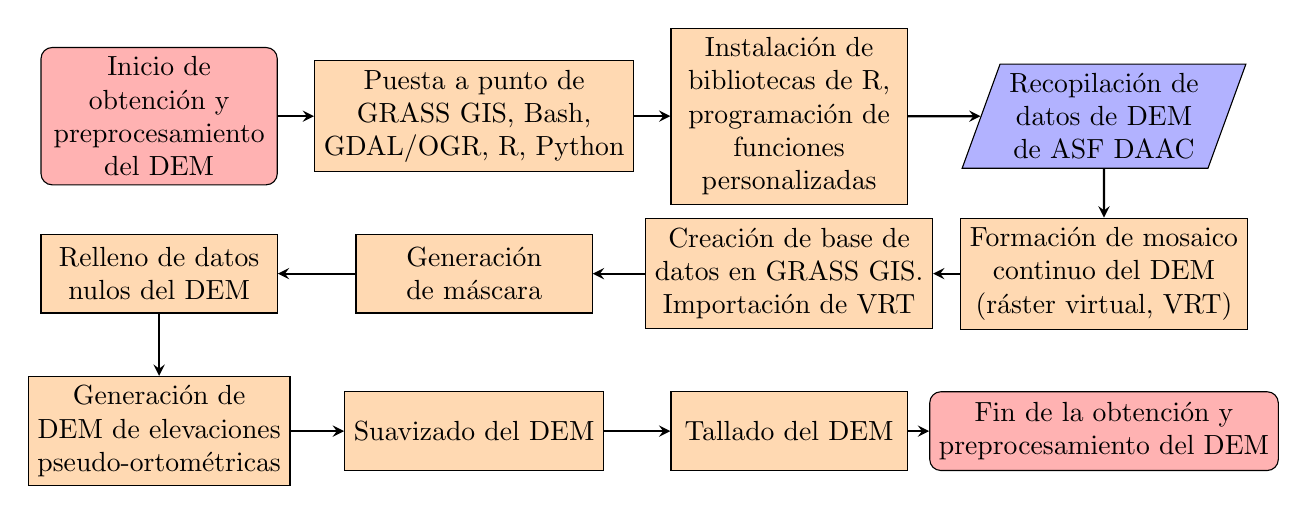
\begin{tikzpicture}[
  startstop/.style={rectangle, rounded corners, minimum width=3cm, minimum height=1cm,text centered, align=center, draw=black, fill=red!30},
  io/.style={trapezium, trapezium left angle=70, trapezium right angle=110, minimum width=3cm, minimum height=1cm, text centered, align=center, draw=black, fill=blue!30},
  process/.style={rectangle, minimum width=3cm, minimum height=1cm, text centered, align=center, draw=black, fill=orange!30},
  decision/.style={diamond, minimum width=3cm, minimum height=1cm, text centered, align=center, draw=black, fill=green!30},
  arrow/.style={thick,->,>=stealth}]

  % Nodes
  \node (start) [startstop] {Inicio de \\ obtención y \\ preprocesamiento \\ del DEM};
  \node (grassgis) [process, right of=start, xshift=3cm] {Puesta a punto de \\ GRASS GIS, Bash, \\ GDAL/OGR, R, Python};
  \node (libreriasR) [process, right of=grassgis, xshift=3cm] {Instalación de \\ bibliotecas de R,\\ programación de \\ funciones \\ personalizadas};
  \node (dataSource) [io, right of=libreriasR, xshift=3cm] {Recopilación de \\ datos de DEM \\ de ASF DAAC};
  \node (mosaic) [process, below of=dataSource, yshift=-1cm] {Formación de mosaico \\ continuo del DEM \\ (ráster virtual, VRT)};
  \node (grassDatabase) [process, left of=mosaic, xshift=-3cm] {Creación de base de \\ datos en GRASS GIS.\\ Importación de VRT};
  \node (mask) [process, left of=grassDatabase, xshift=-3cm] {Generación \\ de máscara};
  \node (fillDEM) [process, left of=mask, xshift=-3cm] {Relleno de datos \\ nulos del DEM};

  \node (pseudoDEM) [process, below of=fillDEM, yshift=-1cm] {Generación de \\ DEM de elevaciones \\ pseudo-ortométricas};
  \node (smoothDEM) [process, right of=pseudoDEM, xshift=3cm] {Suavizado del DEM};
  \node (streamBurn) [process, right of=smoothDEM, xshift=3cm] {Tallado del DEM};
  \node (end) [startstop, right of=streamBurn, xshift=3cm] {Fin de la obtención y \\ preprocesamiento del DEM};

  % Arrows
  \draw [arrow] (start) -- (grassgis);
  \draw [arrow] (grassgis) -- (libreriasR);
  \draw [arrow] (libreriasR) -- (dataSource);

  \draw [arrow] (dataSource) -- (mosaic);
  \draw [arrow] (mosaic) -- (grassDatabase);
  \draw [arrow] (grassDatabase) -- (mask);
  \draw [arrow] (mask) -- (fillDEM);

  \draw [arrow] (fillDEM) -- (pseudoDEM);
  \draw [arrow] (pseudoDEM) -- (smoothDEM);
  \draw [arrow] (smoothDEM) -- (streamBurn);
  \draw [arrow] (streamBurn) -- (end);
\end{tikzpicture}
\end{document}
